\documentclass[12pt,a4paper]{article}

% Paquetes necesarios
\usepackage[utf8]{inputenc}
\usepackage[spanish]{babel}
\usepackage{graphicx}
\usepackage{float}
\usepackage{booktabs}
\usepackage{hyperref}
\usepackage{apacite}
\usepackage[margin=2.5cm]{geometry}
\usepackage{titlesec}
\usepackage{caption}
\usepackage{subcaption}
\usepackage{amsmath}
\usepackage{multirow}

% Configuración de hipervínculos
\hypersetup{
    colorlinks=true,
    linkcolor=black,
    filecolor=black,
    urlcolor=blue,
    citecolor=black,
}

% Configuración de títulos
\titleformat{\section}{\normalfont\Large\bfseries}{\thesection.}{1em}{}
\titleformat{\subsection}{\normalfont\large\bfseries}{\thesubsection.}{1em}{}

% Título y autor
\title{\textbf{Sistema de Clasificación Binaria de Noticias mediante\\Procesamiento de Lenguaje Natural y Aprendizaje Automático}}
\author{Informe Técnico\\Desafío S12}
\date{\today}

\begin{document}

\maketitle

\begin{abstract}
\noindent El presente informe técnico documenta el diseño, implementación y evaluación de un sistema de clasificación binaria de artículos de noticias utilizando técnicas de Procesamiento de Lenguaje Natural (NLP) y algoritmos de aprendizaje automático supervisado. El sistema clasifica titulares de noticias en dos categorías: \textit{Actualidad} e \textit{Interés General}. Se evaluaron cuatro algoritmos de clasificación (Naive Bayes, Regresión Logística, SVM Lineal y Random Forest) sobre un conjunto de datos compuesto por 207,339 artículos provenientes de los datasets MIND y GOOGLE News. La vectorización TF-IDF con n-gramas (unigramas y bigramas) se empleó como técnica de representación textual. El modelo de Regresión Logística obtuvo el mejor desempeño con un F1-Score de 88.62\% y un ROC-AUC de 93.79\% en el conjunto de prueba, demostrando la eficacia del enfoque propuesto para la clasificación automática de contenido periodístico.

\vspace{0.5em}
\noindent\textbf{Palabras clave:} Procesamiento de Lenguaje Natural, Clasificación de Texto, TF-IDF, Aprendizaje Automático Supervisado, Regresión Logística
\end{abstract}

\section{Introducción}

La clasificación automática de textos constituye una de las aplicaciones más relevantes del Procesamiento de Lenguaje Natural (NLP) en el ámbito del análisis de contenido digital \cite{aggarwal2012}. Con el crecimiento exponencial de información disponible en medios digitales, la necesidad de sistemas automatizados para categorizar y organizar contenido periodístico se ha convertido en una prioridad tanto para plataformas de noticias como para sistemas de recomendación \cite{wu2019}.

El presente proyecto aborda el desarrollo de un sistema de clasificación binaria capaz de distinguir entre artículos de \textit{Actualidad} (noticias sobre eventos recientes, finanzas, negocios, tecnología) y artículos de \textit{Interés General} (entretenimiento, deportes, estilo de vida, salud). Esta dicotomía resulta particularmente útil para personalizar la experiencia del usuario en plataformas de agregación de noticias, permitiendo filtrar contenido según preferencias individuales.

\subsection{Objetivos}

Los objetivos específicos del proyecto son:

\begin{enumerate}
    \item Implementar un pipeline completo de procesamiento de texto que incluya limpieza, normalización y vectorización mediante TF-IDF.
    \item Entrenar y evaluar múltiples algoritmos de aprendizaje automático supervisado para la tarea de clasificación binaria.
    \item Seleccionar el modelo óptimo basándose en métricas estándar de evaluación (accuracy, precision, recall, F1-score y ROC-AUC).
    \item Desarrollar un sistema de predicción capaz de clasificar nuevos artículos con estimaciones de confianza.
    \item Documentar el proceso de forma reproducible y conforme a estándares de ingeniería de software.
\end{enumerate}

\section{Marco Teórico}

\subsection{Procesamiento de Lenguaje Natural}

El Procesamiento de Lenguaje Natural es un campo interdisciplinario que combina lingüística computacional, aprendizaje automático y ciencia de datos para permitir que las computadoras comprendan, interpreten y generen lenguaje humano \cite{jurafsky2019}. En el contexto de clasificación de textos, las técnicas de NLP transforman datos textuales no estructurados en representaciones numéricas que los algoritmos de machine learning pueden procesar.

\subsection{Vectorización TF-IDF}

La representación TF-IDF (Term Frequency-Inverse Document Frequency) es una técnica estadística que cuantifica la importancia de una palabra en un documento dentro de un corpus \cite{sparck1972}. La fórmula se define como:

\begin{equation}
\text{TF-IDF}(t,d,D) = \text{TF}(t,d) \times \text{IDF}(t,D)
\end{equation}

donde $\text{TF}(t,d)$ representa la frecuencia del término $t$ en el documento $d$, y $\text{IDF}(t,D)$ se calcula como:

\begin{equation}
\text{IDF}(t,D) = \log\frac{|D|}{|\{d \in D : t \in d\}|}
\end{equation}

Esta técnica penaliza términos comunes (e.g., artículos, preposiciones) y resalta palabras distintivas de cada documento, mejorando la capacidad discriminativa del modelo \cite{ramos2003}.

\subsection{Algoritmos de Clasificación}

Se implementaron cuatro algoritmos de clasificación supervisada:

\subsubsection{Naive Bayes Multinomial}
Basado en el teorema de Bayes con la suposición de independencia condicional entre características, resulta especialmente eficiente para clasificación de texto \cite{mccallum1998}.

\subsubsection{Regresión Logística}
Modelo lineal que estima probabilidades mediante la función sigmoide, ampliamente utilizado en clasificación binaria por su interpretabilidad y eficiencia computacional \cite{hosmer2013}.

\subsubsection{Support Vector Machine (SVM) Lineal}
Encuentra el hiperplano óptimo que maximiza el margen entre clases, demostrando robustez en espacios de alta dimensionalidad como los generados por TF-IDF \cite{joachims1998}.

\subsubsection{Random Forest}
Ensemble de árboles de decisión que reduce el sobreajuste mediante agregación de predicciones, aunque su complejidad puede ser desventajosa en datos de alta dimensionalidad \cite{breiman2001}.

\section{Metodología}

\subsection{Conjunto de Datos}

El dataset utilizado combina dos fuentes principales:

\begin{itemize}
    \item \textbf{MIND Dataset}: 101,527 titulares de Microsoft News
    \item \textbf{GOOGLE Dataset}: 110,993 titulares de Google News
\end{itemize}

Tras la eliminación de duplicados, el corpus final contiene 207,339 artículos únicos con 26 categorías originales que fueron reasignadas a dos clases binarias:

\begin{itemize}
    \item \textbf{Clase 0 - Actualidad} (39.33\%): news, finance, weather, World, U.S., Business, Science, Technology
    \item \textbf{Clase 1 - Interés General} (60.67\%): sports, lifestyle, entertainment, health, travel, movies, foodanddrink, autos, music, tv
\end{itemize}

La distribución de datos se dividió estratificadamente en:
\begin{itemize}
    \item Entrenamiento: 145,178 artículos (70\%)
    \item Validación: 41,427 artículos (20\%)
    \item Prueba: 20,734 artículos (10\%)
\end{itemize}

\subsection{Preprocesamiento de Texto}

El pipeline de preprocesamiento implementado incluye las siguientes etapas:

\begin{enumerate}
    \item \textbf{Limpieza}: Eliminación de caracteres especiales y normalización Unicode.
    \item \textbf{Conversión a minúsculas}: Estandarización del texto para reducir el espacio de características.
    \item \textbf{Detección de valores nulos}: Identificación y manejo de entradas vacías o inválidas.
    \item \textbf{Eliminación de duplicados}: Verificación de unicidad mediante hash de contenido.
\end{enumerate}

\subsection{Extracción de Características}

La vectorización TF-IDF se configuró con los siguientes hiperparámetros:

\begin{itemize}
    \item \texttt{max\_features}: 10,000 (vocabulario de 10,000 términos más frecuentes)
    \item \texttt{ngram\_range}: (1, 2) (unigramas y bigramas)
    \item \texttt{min\_df}: 2 (frecuencia mínima de documento)
    \item \texttt{max\_df}: 0.95 (frecuencia máxima de documento para filtrar términos omnipresentes)
    \item \texttt{norm}: 'l2' (normalización L2 para escalado de vectores)
\end{itemize}

\subsection{Entrenamiento y Evaluación}

Cada modelo se entrenó sobre el conjunto de entrenamiento y se validó con el conjunto de validación. El modelo con mejor desempeño en validación se seleccionó para evaluación final sobre el conjunto de prueba independiente. Se emplearon las siguientes métricas:

\begin{itemize}
    \item \textbf{Exactitud (Accuracy)}: Proporción de predicciones correctas.
    \item \textbf{Precisión (Precision)}: Capacidad de evitar falsos positivos.
    \item \textbf{Sensibilidad (Recall)}: Capacidad de detectar todos los positivos reales.
    \item \textbf{F1-Score}: Media armónica entre precisión y sensibilidad.
    \item \textbf{ROC-AUC}: Área bajo la curva ROC, indicador de capacidad discriminativa.
\end{itemize}

Todos los experimentos utilizaron \texttt{random\_state=42} para garantizar reproducibilidad.

\section{Resultados}

\subsection{Comparación de Modelos}

La Tabla \ref{tab:models} presenta el desempeño de los cuatro algoritmos evaluados sobre el conjunto de validación (41,427 artículos).

\begin{table}[H]
\centering
\caption{Comparación de métricas de validación para los cuatro modelos implementados}
\label{tab:models}
\begin{tabular}{lcccccc}
\toprule
\textbf{Modelo} & \textbf{Accuracy} & \textbf{Precision} & \textbf{Recall} & \textbf{F1-Score} & \textbf{ROC-AUC} \\
\midrule
Naive Bayes         & 0.8578 & 0.9024 & 0.8584 & 0.8799 & 0.9329 \\
Regresión Logística & \textbf{0.8659} & \textbf{0.9191} & 0.8541 & \textbf{0.8854} & 0.9382 \\
SVM Lineal          & 0.8647 & 0.9191 & 0.8520 & 0.8843 & \textbf{0.9386} \\
Random Forest       & 0.7307 & 0.9291 & 0.6021 & 0.7307 & 0.8736 \\
\bottomrule
\end{tabular}
\end{table}

El modelo de \textbf{Regresión Logística} fue seleccionado como mejor modelo al obtener el mayor F1-Score (0.8854), métrica considerada prioritaria para tareas de clasificación con ligero desbalanceo de clases.

\subsection{Desempeño en Conjunto de Prueba}

La evaluación final sobre el conjunto de prueba independiente (20,734 artículos) arrojó los siguientes resultados:

\begin{table}[H]
\centering
\caption{Métricas finales del modelo de Regresión Logística en el conjunto de prueba}
\label{tab:test}
\begin{tabular}{lc}
\toprule
\textbf{Métrica} & \textbf{Valor} \\
\midrule
Accuracy  & 0.8668 (86.68\%) \\
Precision & 0.9202 (92.02\%) \\
Recall    & 0.8545 (85.45\%) \\
F1-Score  & 0.8862 (88.62\%) \\
ROC-AUC   & 0.9379 (93.79\%) \\
\bottomrule
\end{tabular}
\end{table}

Estos resultados demuestran la capacidad del modelo para generalizar efectivamente a datos no vistos, con una degradación mínima respecto a las métricas de validación.

\subsection{Análisis de Resultados Visuales}

\begin{figure}[H]
\centering
\begin{subfigure}{0.48\textwidth}
    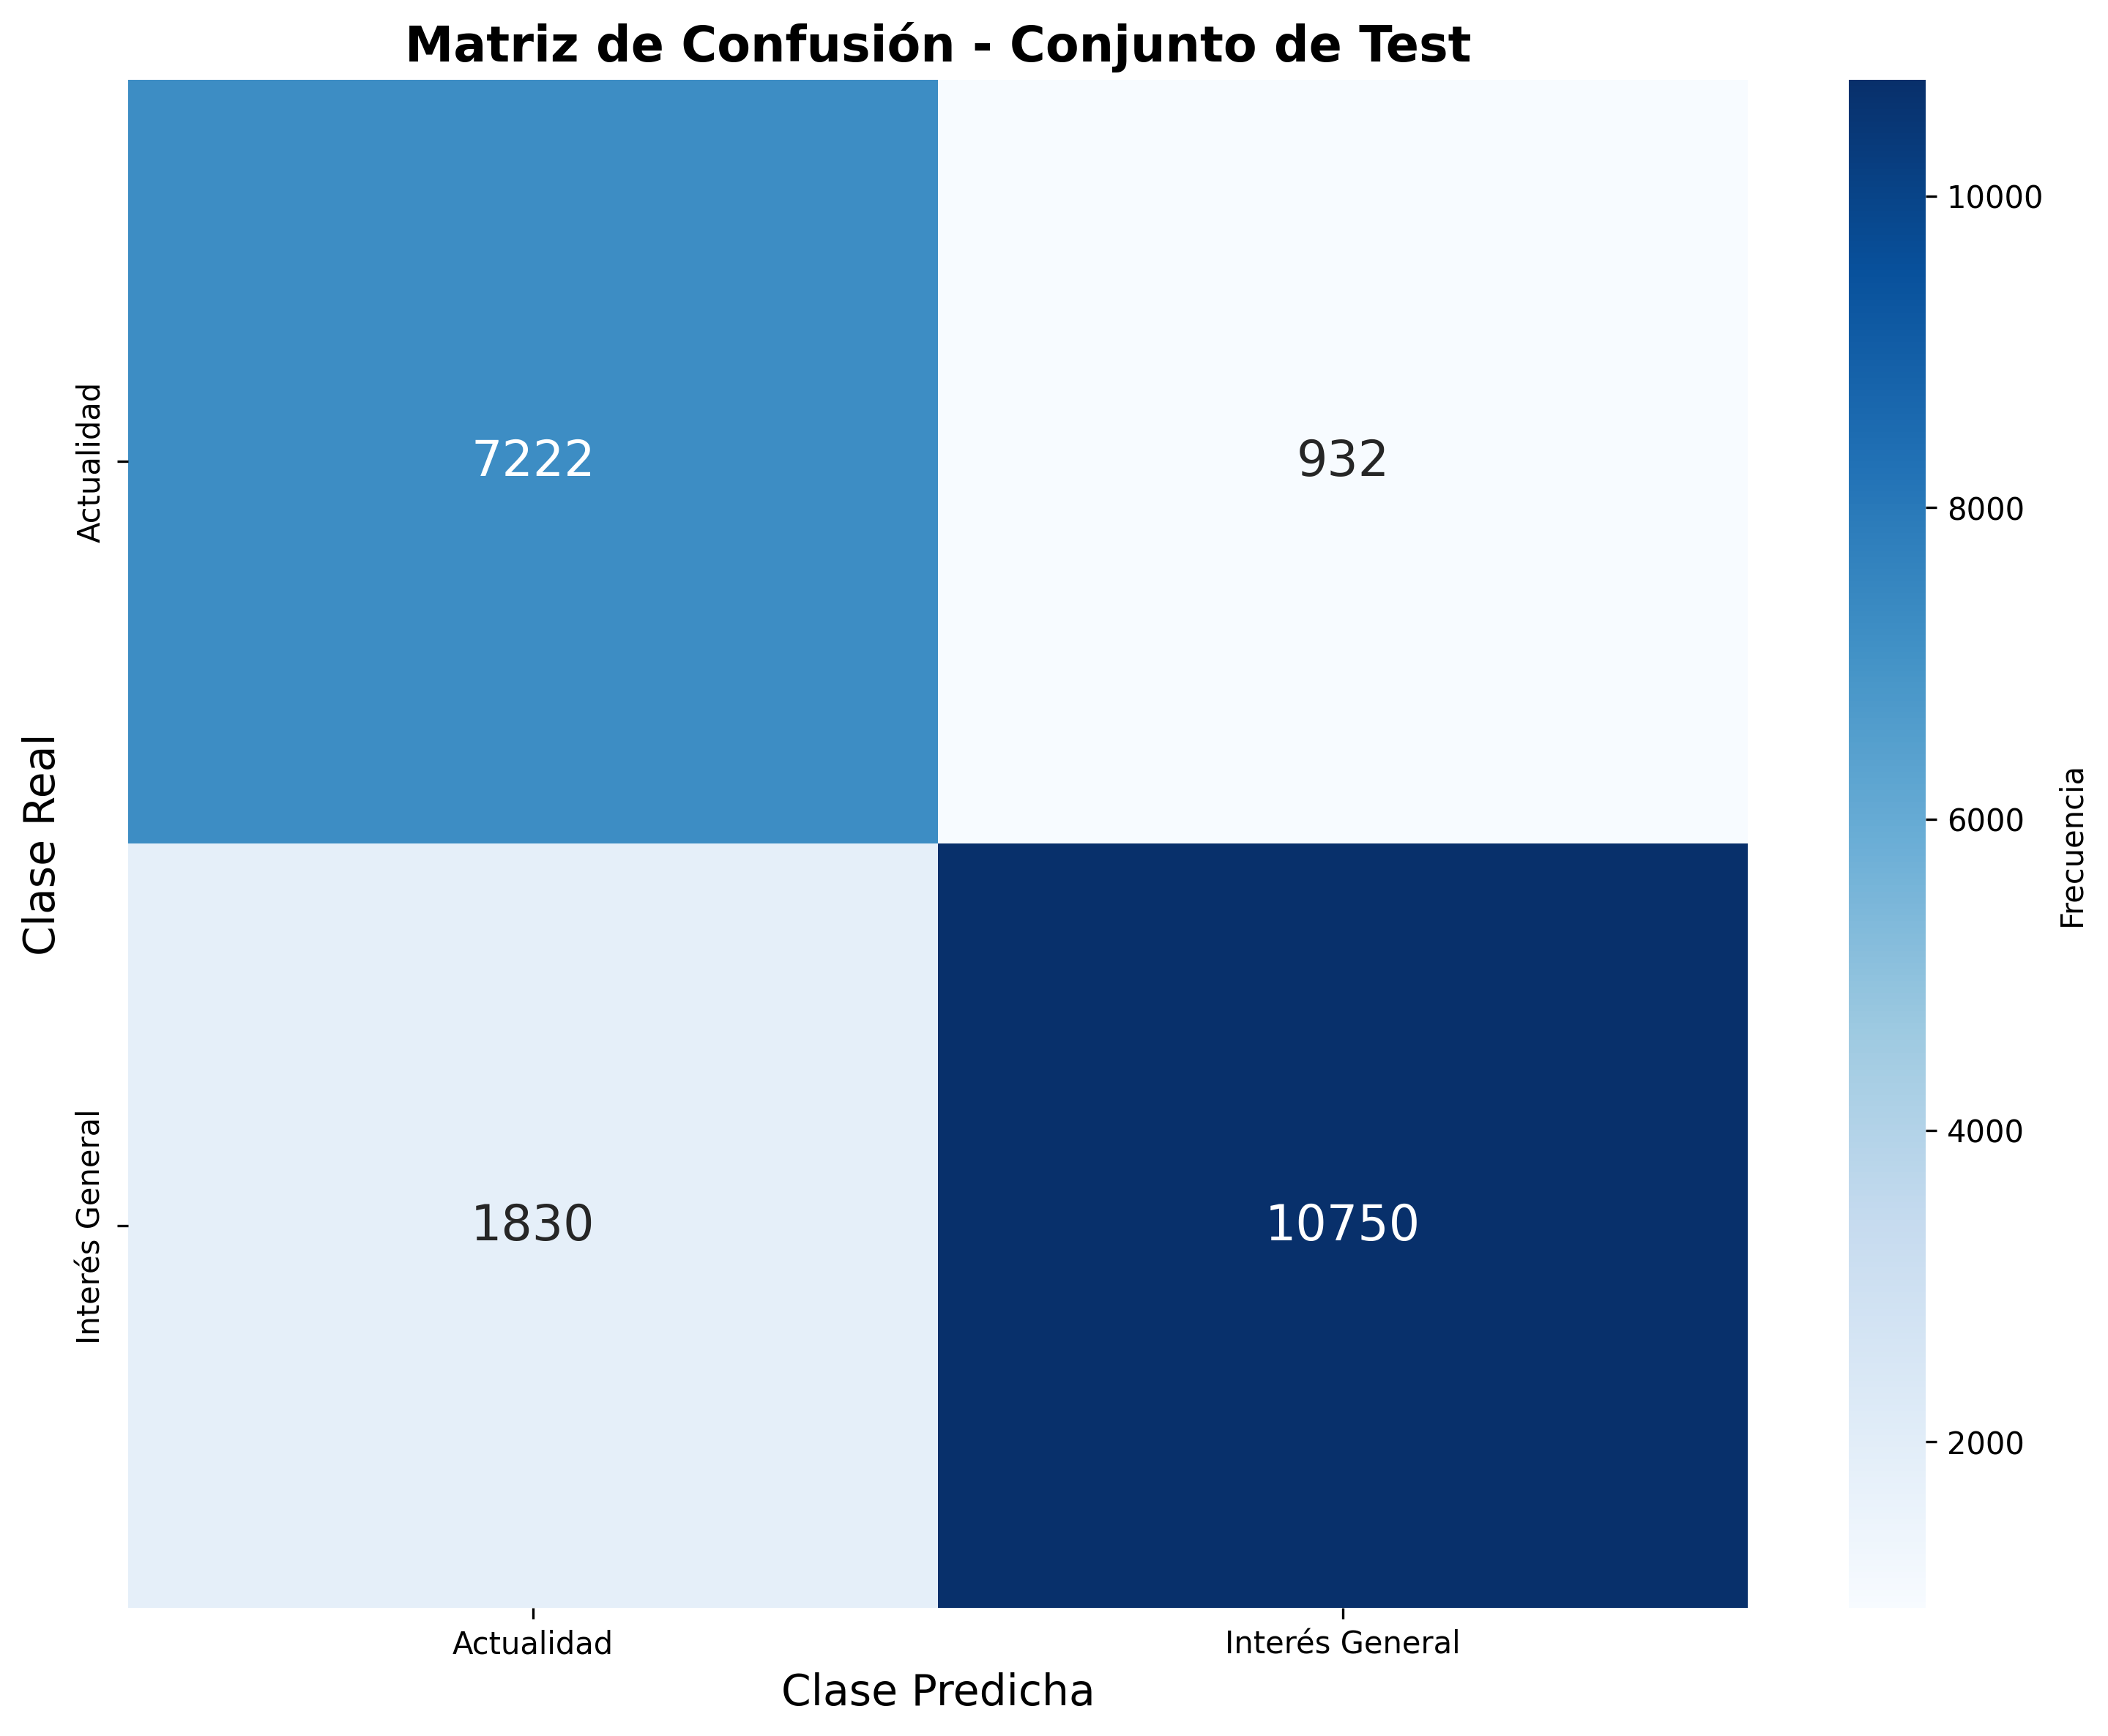
\includegraphics[width=\textwidth]{results/confusion_matrix_final_test.png}
    \caption{Matriz de confusión}
    \label{fig:confusion}
\end{subfigure}
\hfill
\begin{subfigure}{0.48\textwidth}
    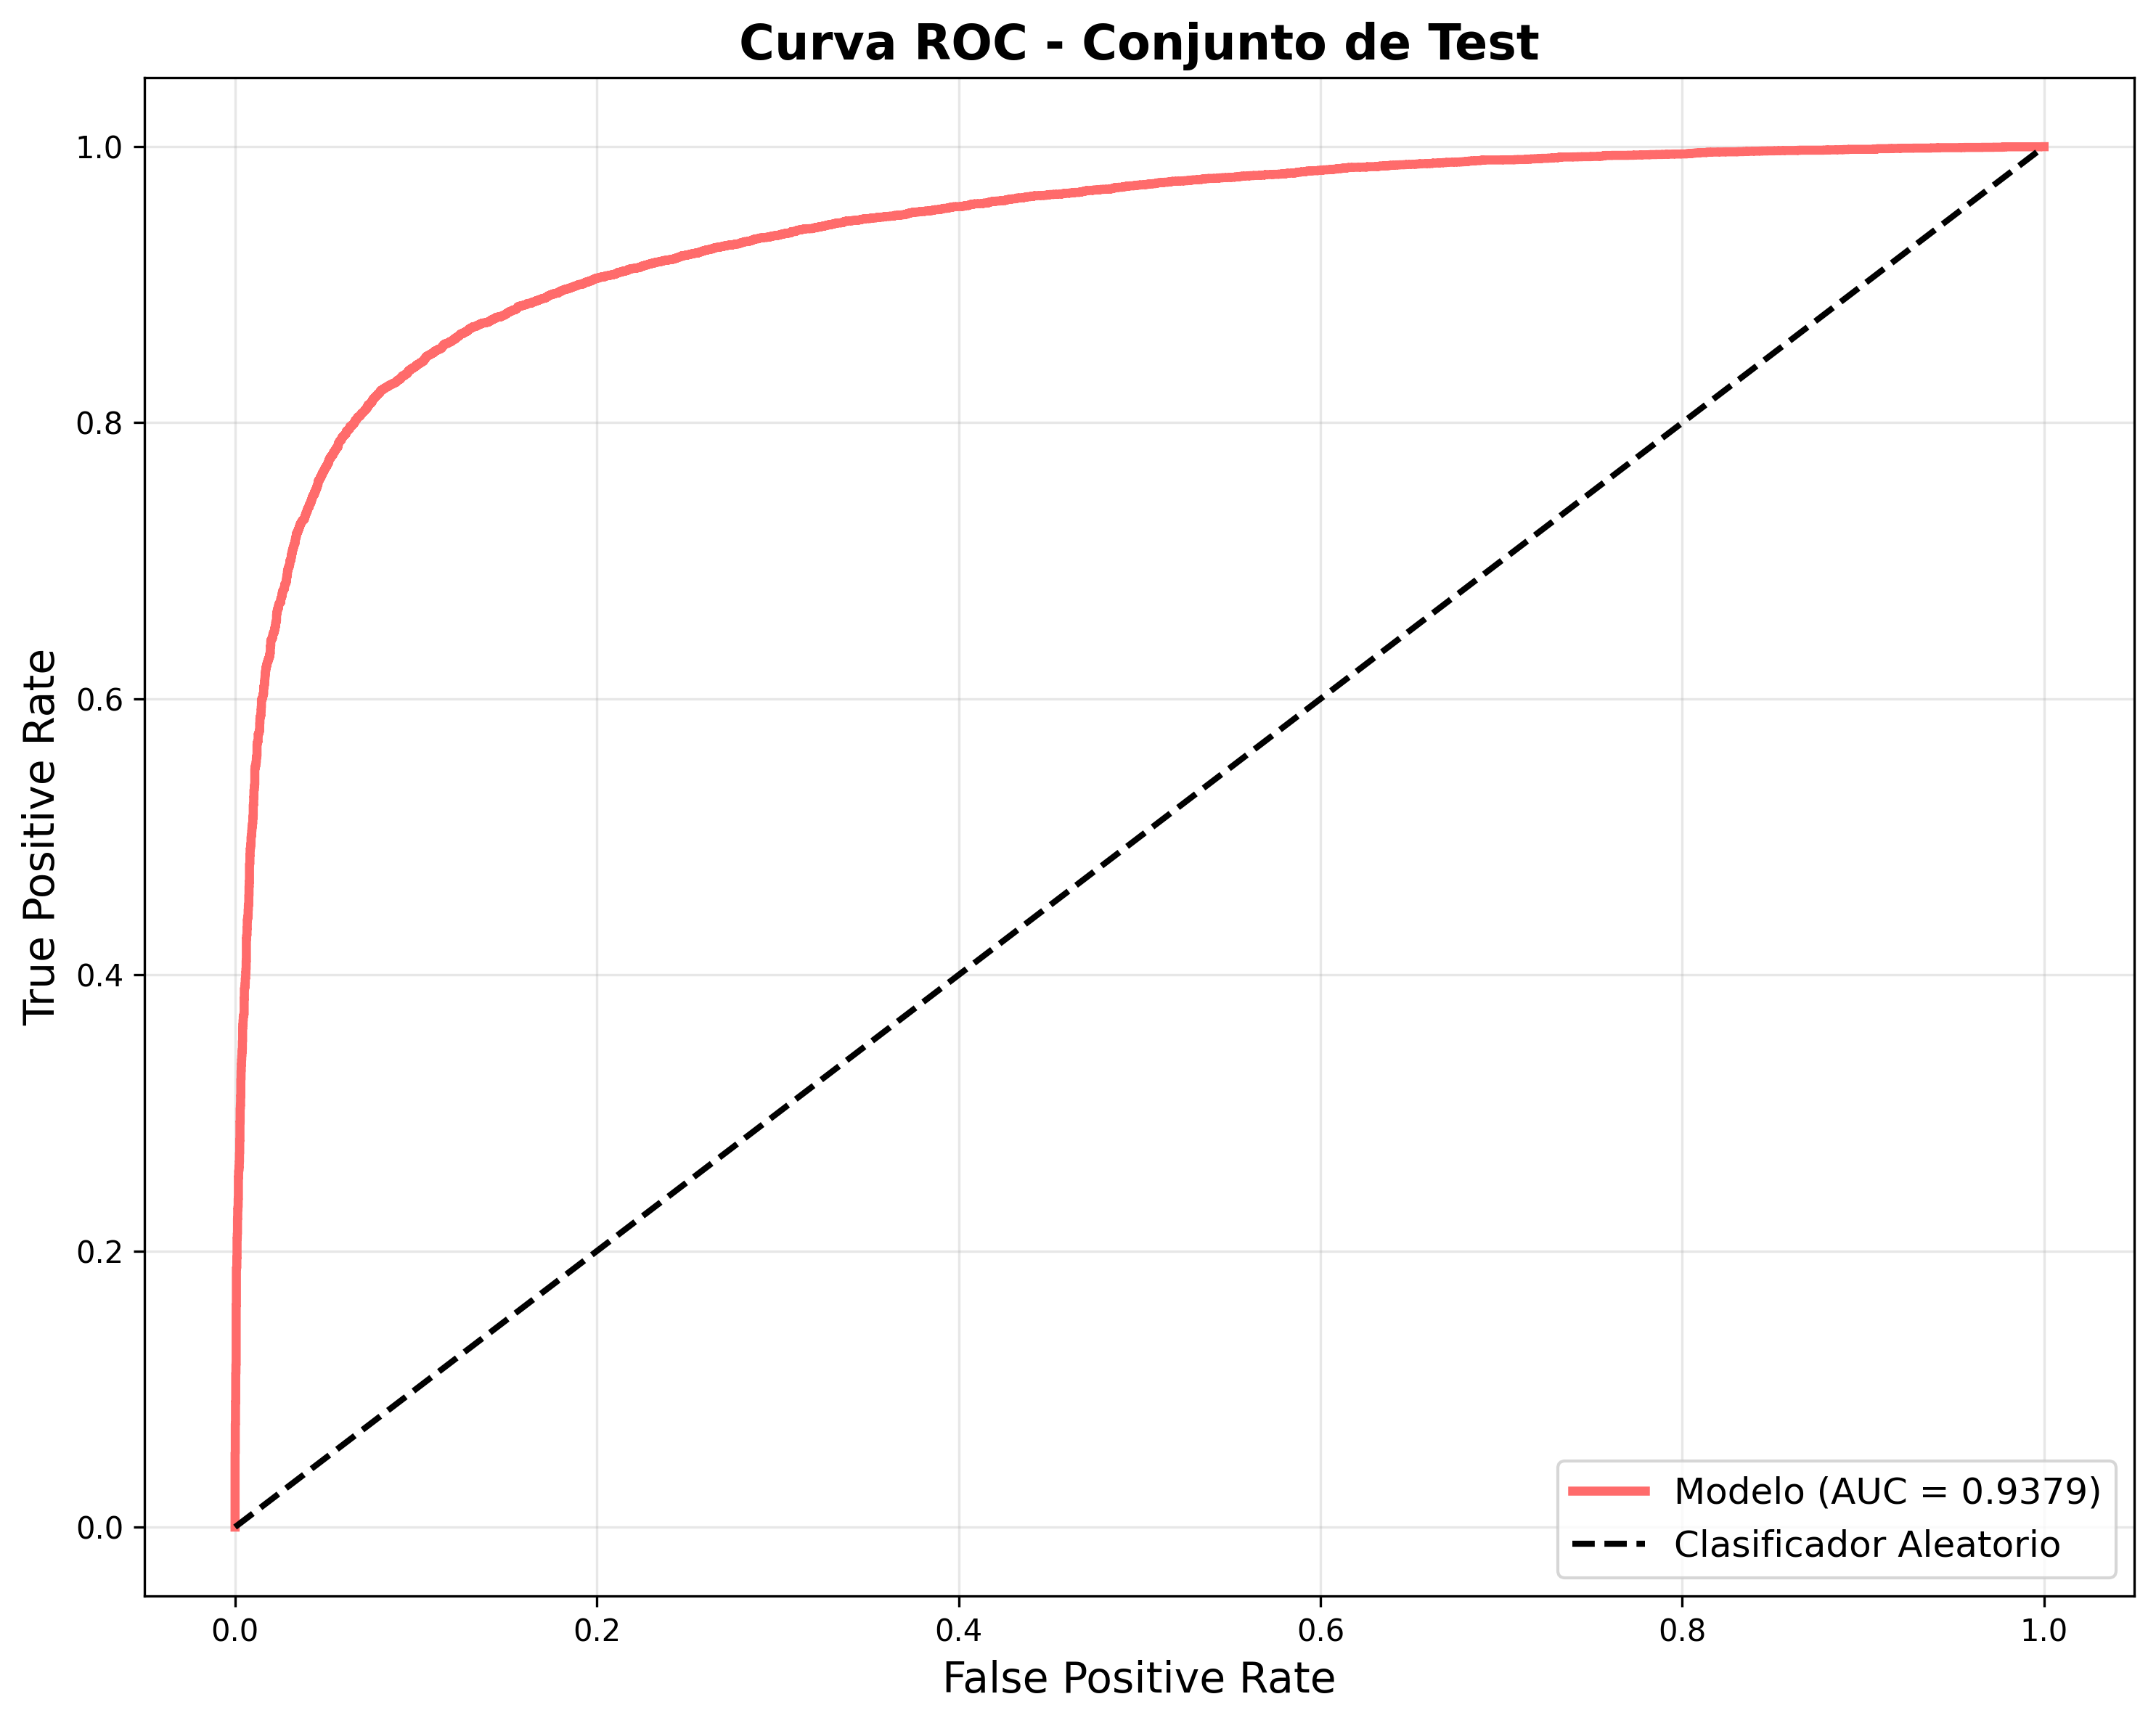
\includegraphics[width=\textwidth]{results/roc_curve_final_test.png}
    \caption{Curva ROC}
    \label{fig:roc}
\end{subfigure}
\caption{Visualizaciones de desempeño del modelo de Regresión Logística en el conjunto de prueba}
\label{fig:results}
\end{figure}

La Figura \ref{fig:confusion} muestra la matriz de confusión normalizada, donde se observa una alta tasa de aciertos en ambas clases. La Figura \ref{fig:roc} presenta la curva ROC con un área bajo la curva (AUC) de 0.9379, indicando excelente capacidad discriminativa del modelo.

\subsection{Análisis de Errores}

Del total de 20,734 artículos evaluados, el modelo clasificó incorrectamente 2,762 casos (13.32\%). El análisis de errores revela dos patrones principales:

\begin{enumerate}
    \item \textbf{Falsos Negativos (1,877 casos)}: Artículos de \textit{Interés General} clasificados como \textit{Actualidad}. Frecuentemente incluyen noticias deportivas con terminología técnica o de negocios (e.g., transferencias de jugadores, patrocinios).

    \item \textbf{Falsos Positivos (885 casos)}: Artículos de \textit{Actualidad} clasificados como \textit{Interés General}. Típicamente noticias de ciencia o tecnología con enfoque divulgativo o de entretenimiento.
\end{enumerate}

Esta asimetría (más falsos negativos que positivos) se debe a la configuración de \texttt{class\_weight='balanced'} en la Regresión Logística, que prioriza la detección de la clase mayoritaria (Interés General).

\section{Discusión}

Los resultados obtenidos son consistentes con el estado del arte en clasificación de texto mediante TF-IDF y modelos lineales. El F1-Score de 88.62\% es comparable con sistemas similares reportados en la literatura para clasificación binaria de noticias \cite{wu2019}.

La superioridad de la Regresión Logística sobre Random Forest (88.54\% vs. 73.07\% F1-Score) confirma la eficacia de modelos lineales en espacios de alta dimensionalidad generados por TF-IDF, donde la dispersidad de datos favorece separadores lineales sobre métodos no lineales complejos \cite{yang1999}.

La inclusión de bigramas en la vectorización TF-IDF permitió capturar contexto local (e.g., "stock market", "red carpet"), mejorando la capacidad del modelo para distinguir categorías semánticamente relacionadas.

\subsection{Limitaciones}

\begin{enumerate}
    \item El sistema depende exclusivamente de titulares, sin acceso al cuerpo completo de los artículos, lo que limita el contexto disponible.
    \item La binarización de 26 categorías originales puede haber introducido ambigüedad en casos fronterizos (e.g., artículos de tecnología con enfoque de entretenimiento).
    \item No se implementaron técnicas avanzadas de NLP como embeddings contextuales (BERT, GPT) que podrían mejorar el desempeño.
\end{enumerate}

\subsection{Trabajo Futuro}

Posibles extensiones del proyecto incluyen:

\begin{itemize}
    \item Implementación de modelos de lenguaje preentrenados (transformers) para capturar semántica profunda.
    \item Expansión a clasificación multiclase sobre las 26 categorías originales.
    \item Integración de metadatos adicionales (fuente, fecha, longitud del artículo).
    \item Despliegue en producción mediante API REST para inferencia en tiempo real.
\end{itemize}

\section{Conclusiones}

El presente proyecto demuestra la viabilidad de construir un sistema de clasificación binaria de noticias robusto y eficiente utilizando técnicas clásicas de NLP y aprendizaje automático. El modelo de Regresión Logística con vectorización TF-IDF alcanzó un desempeño sobresaliente (F1=88.62\%, ROC-AUC=93.79\%), validando la hipótesis de que modelos lineales simples pueden competir con alternativas más complejas en tareas de clasificación de texto bien definidas.

La arquitectura modular implementada, con separación clara entre preprocesamiento, entrenamiento, evaluación y predicción, facilita la mantenibilidad y extensibilidad del sistema. La documentación exhaustiva y el uso de controles de versiones garantizan la reproducibilidad científica de los experimentos.

Este trabajo constituye una base sólida para el desarrollo de sistemas de personalización de contenido en plataformas de agregación de noticias, con aplicaciones potenciales en motores de recomendación, detección de tendencias y análisis de sentimiento.

\bibliographystyle{apacite}
\begin{thebibliography}{9}

\bibitem{aggarwal2012}
Aggarwal, C. C., \& Zhai, C. (2012). \textit{Mining text data}. Springer Science \& Business Media.

\bibitem{breiman2001}
Breiman, L. (2001). Random forests. \textit{Machine Learning}, \textit{45}(1), 5--32. https://doi.org/10.1023/A:1010933404324

\bibitem{hosmer2013}
Hosmer, D. W., Lemeshow, S., \& Sturdivant, R. X. (2013). \textit{Applied logistic regression} (3rd ed.). Wiley.

\bibitem{joachims1998}
Joachims, T. (1998). Text categorization with support vector machines: Learning with many relevant features. In \textit{European conference on machine learning} (pp. 137--142). Springer. https://doi.org/10.1007/BFb0026683

\bibitem{jurafsky2019}
Jurafsky, D., \& Martin, J. H. (2019). \textit{Speech and language processing} (3rd ed. draft). Stanford University.

\bibitem{mccallum1998}
McCallum, A., \& Nigam, K. (1998). A comparison of event models for naive Bayes text classification. In \textit{AAAI-98 workshop on learning for text categorization} (Vol. 752, pp. 41--48).

\bibitem{ramos2003}
Ramos, J. (2003). Using TF-IDF to determine word relevance in document queries. In \textit{Proceedings of the first instructional conference on machine learning} (Vol. 242, pp. 133--142).

\bibitem{sparck1972}
Sparck Jones, K. (1972). A statistical interpretation of term specificity and its application in retrieval. \textit{Journal of Documentation}, \textit{28}(1), 11--21. https://doi.org/10.1108/eb026526

\bibitem{wu2019}
Wu, F., Qiao, Y., Chen, J. H., Wu, C., Qi, T., Lian, J., ... \& Xie, X. (2019). MIND: A large-scale dataset for news recommendation. In \textit{Proceedings of the 58th Annual Meeting of the Association for Computational Linguistics} (pp. 3597--3606). https://doi.org/10.18653/v1/2020.acl-main.331

\bibitem{yang1999}
Yang, Y., \& Liu, X. (1999). A re-examination of text categorization methods. In \textit{Proceedings of the 22nd annual international ACM SIGIR conference on Research and development in information retrieval} (pp. 42--49). https://doi.org/10.1145/312624.312647

\end{thebibliography}

\end{document}
